\documentclass[letterpaper, 12 pt, onecolumn, hidelinks]{ieeetran}
\IEEEoverridecommandlockouts

\usepackage[margin=1in]{geometry}
\usepackage{microtype,xparse,tcolorbox}
\usepackage{mathtools, cuted}
\usepackage{todonotes}
\usepackage{graphicx}
\usepackage{wrapfig}
\usepackage{hyperref}
\usepackage{overpic}
\usepackage{wrapfig}
\graphicspath{{./pictures/}}

\begin{document}
\thispagestyle{empty}\vspace*{\fill} {\centering {\large University of Houston -  Cullen College of Engineering\\\vspace{1.25cm}{\LARGE \bf Project Stride:\\\medspace Energy Generating Shoes}\\\vspace{1.5cm} Team 7\\Robert Duenez, Denny Luong, \emph{Lillian Lin}, and Pavani Tenneti\\\vspace{1.25cm}Sponsor: Doug Varret\\}}
\vspace*{\fill} 

\break

\thispagestyle{empty}\vspace*{\fill} 

\begin{quote}  	
	Lillian Lin\\Chief Technical Officer, Project Stride\\4800 Calhoun Rd\\Houston, TX 77004\\Email: lklin@uh.edu\\Phone: (409) 293 - 5277\vspace{0.5cm} \\
	\today \vspace{0.5cm}\\
	Dr.\ Steven Pei,\\
	Facilitator, ECE 4335 Capstone Design\\
	W322 Engineering Building 2\\
	Houston, TX 77004
	\vspace{2cm} \\
	
	Dear Dr.\ Steven Pei,\medskip\\
	Please find attached the report for team 7, Project Stride: Energy Generating Shoes. In this report we describe the progress with respect to our timelines, highlight the testing procedures we have designed, determine if we are meeting engineering standards, and discuss our upcoming goals. Please let us know if further information is required. Your consideration is greatly appreciated.\vspace{0.5cm}\\
	Sincerely,\\
	
	
\includegraphics[width=4cm]{LilliansSignature.png}
	\medskip\\
	Lillian Lin 
\end{quote}
\setcounter{page}{0}\vspace*{\fill}
\break

\section*{Abstract}
Project Stride strives to provide a means for caretakers to have peace of mind while offering users freedom in the form of a location reporting shoe that is completely sustained on the kinetic energy a human generates by walking. Our project

\break

\section{Purpose}\label{sec:Purpose}
This report describes our project details and progress made towards achieving our goals. This includes a background and summary of the project, the target objective and goals planned to meet our target objective, as well as constraints and specifications we will be considering while making our design. The report will also briefly discuss the budget and risk minimization needed for the project.

\section{Background}\label{sec:Background}
Each year 125,000 search and rescue missions are done to locate Alzheimer patients. The National Park Services have reported over \$5 million and hundreds of thousands of hours in annual costs for search across the United States. This issue could be solved if there was a reliable way to know the location of those who are prone to getting lost, people with disabilities, elderly with memory issues, and children. 

Enter, Project Stride. Project Stride proposes a low power system that automatically logs the users location from the sole of their shoe with no other equipment required. This location wireless transfers to a caretakers phone and alerts this phone of the user's location when they get outside a specified area. All of this is powered solely by the energy generated by walking, leaving the caretaker without worry that the device will run out of battery life.

\section{Overview}\label{sec:Overview}
The project we are designing is an incredibly low powered system and can be considered to only have two main systems, the energy system and the data transfer system. This flow can be seen in Fig. \ref{fig:Diagram}, where green arrows represent the flow of energy and blue arrows represent the flow of information.

\begin{figure}[h]
	\begin{center}
		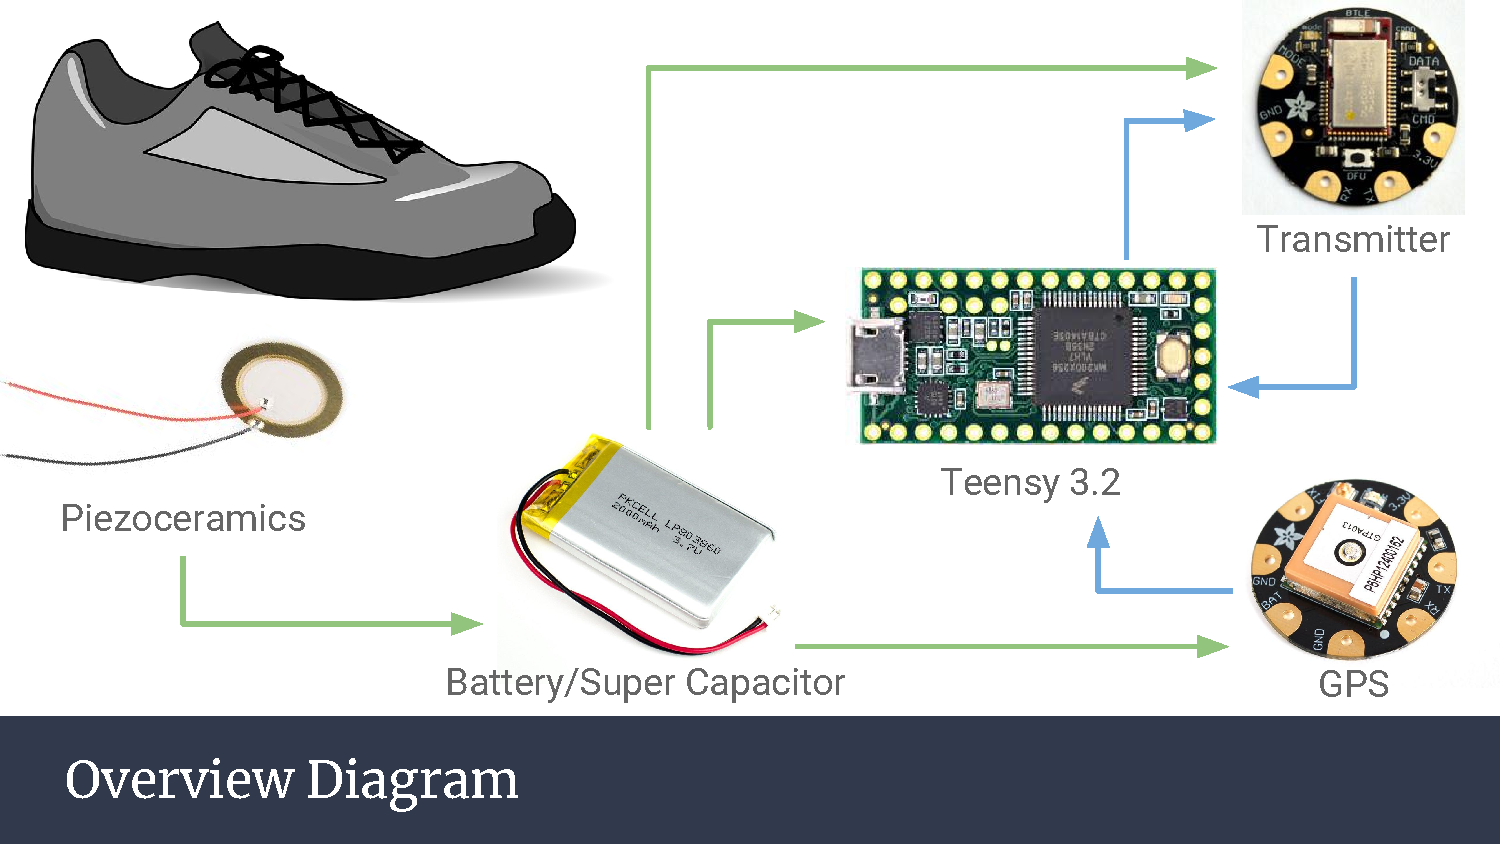
\includegraphics[trim=0 65 0 0, clip, width=\columnwidth]{OverviewDiagram.pdf}
	\end{center}
	\vspace{-1em}
	\caption{\label{fig:Diagram}Goal Analysis for the Entire Year}
\end{figure}

The energy system is centered around the use of piezoceramic disks as a means to convert kinetic energy from walking into electrical energy. As piezo ceramics are known for generating a voltage whenever pressure is applied to them, this voltage will then be harvested into an energy bank taking the form of either a battery or super capacitor. The energy then feeds into the transmitter, microprocessor, and GPS module.

The microprocessor will be used as a means to interpret location data from the GPS. This location data is then send to the transmitter when the microprocessor determines that the user is no longer within a specified area or if the transmitter receives a request from a cell phone for the location data. While this transmitter is intended to be a long range antenna for use without a cell phone, for testing purposes we will be using a bluetooth module.

\section{Goal Analysis}\label{sec:Goal}
Our target objective for this project is to create a shoe that will be able to convert kinetic energy made by walking into usable electrical energy. This energy will power a microcontroller that will relay the location of the user's shoe to an android app on another user's phone. In order to reach this target objective, subgoals have been defined as seen in Fig. \ref{fig:Flowchart} to create benchmarks for progress.

\begin{figure}[h]
	\begin{center}
		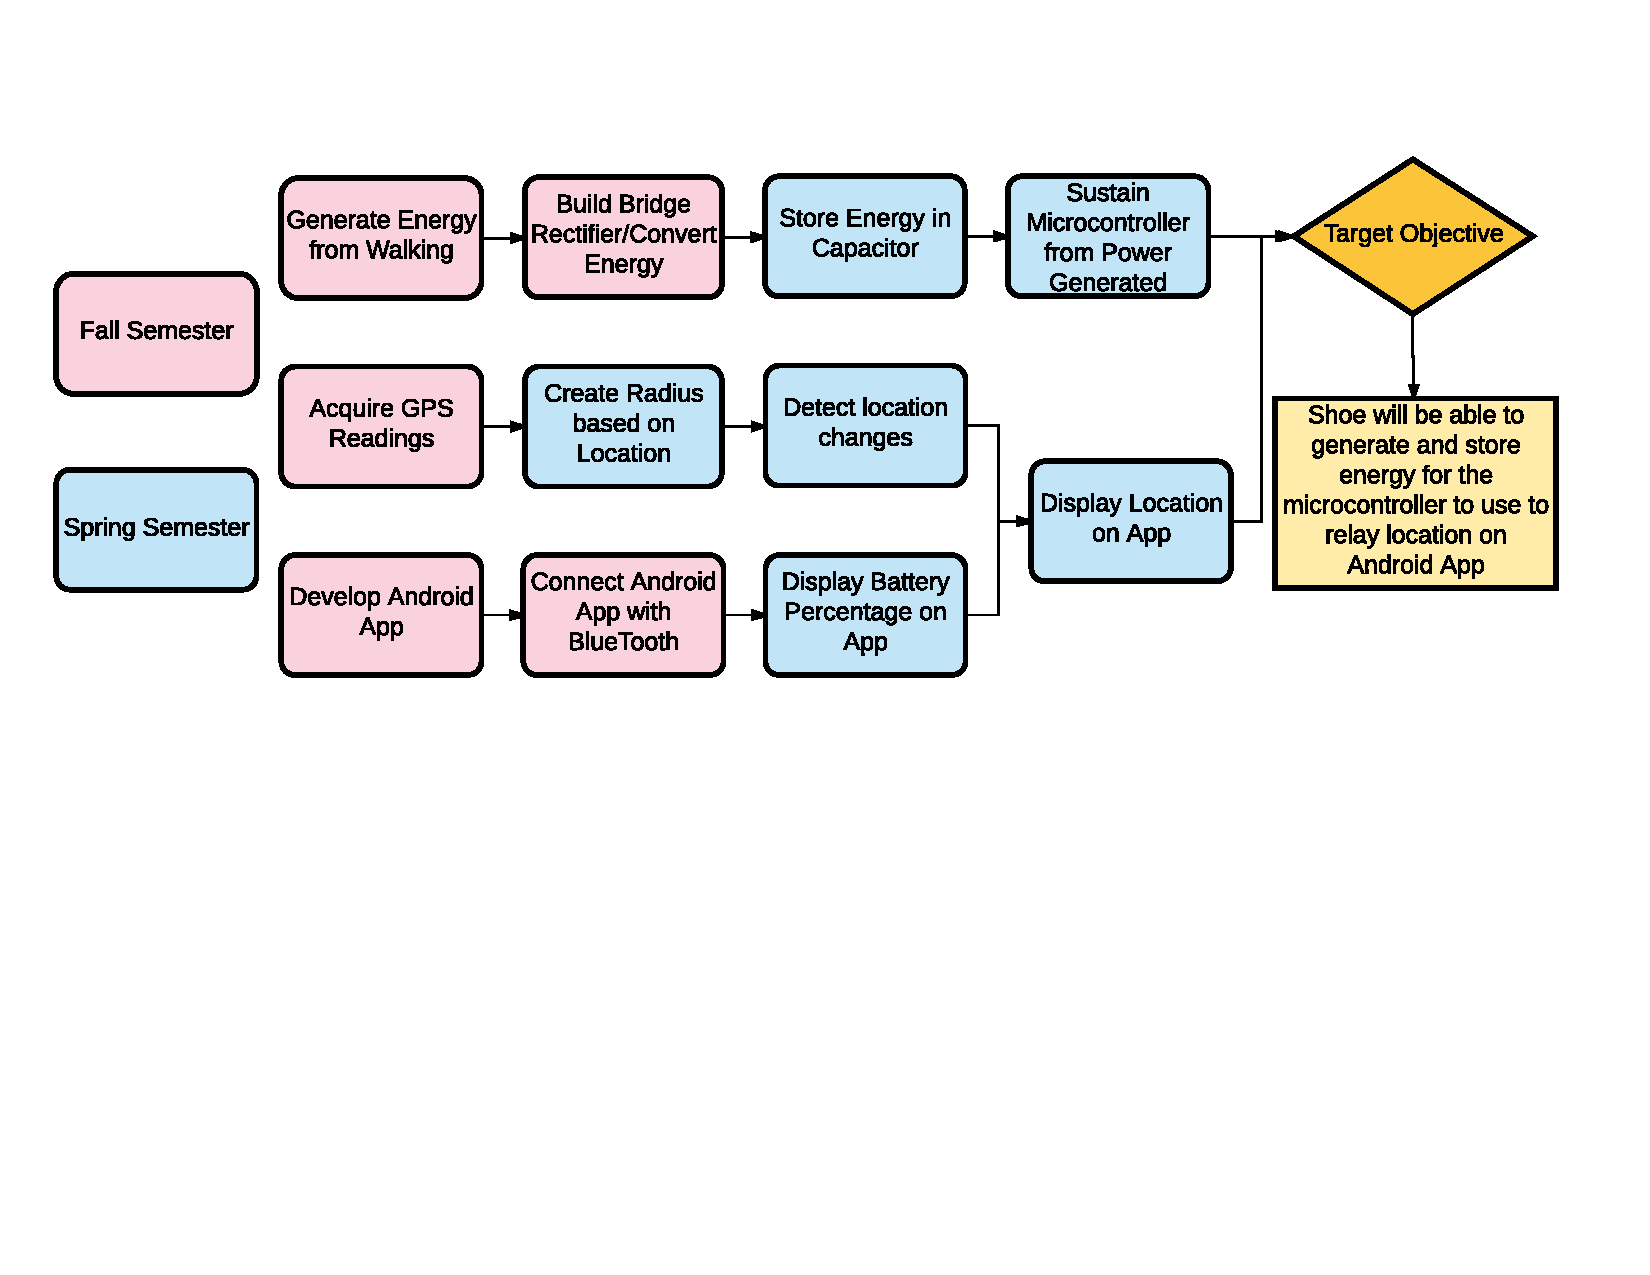
\includegraphics[trim=25 275 40 75, clip, width=\columnwidth]{ProjectStrideGoalAnaylsis.pdf}
	\end{center}
	\vspace{-1em}
	\caption{\label{fig:Flowchart}Goal Analysis for the Entire Year}
\end{figure}

The first and current semester, highlighted in pink, will work on hardware capabilities of the system. This includes generating energy, determining an energy threshold for data transfer and ensuring that all sensors are functional. While currently parts are being used for testing, it is still possible for these to changed based on the amount of energy the system can provide. The second semester will work on software and reliability.

\section{Engineering Standards and Constraints}\label{sec:Standards}

I don't know what to put here about standards guys so I'd love some input please and thank you. I thought about leaving this blank but I can see if you actually read it if you respond to this part since it's obviously not really text if you read it. I should probably write something about not killing people since 9/10 most people don't buy something if it catches you on fire.

As this system will be working with piezoceramics as the method of generating energy, this will restrict the entire system to operate in a low energy state since, despite the piezoceramics making a noticeable voltage spike, the current from most piezoceramics are in the milliampere range. This means the available energy to harvest is in the milliwatts.

Another main constraint with our system is the usable workspace inside the shoe. Although the end goal is to completely replace the shoe sole with a Project Stride sole, the average shoe only gives a 1 centimeter depth of workspace for a circuit to operate in and requires a flexible enough material to allow the person wearing it to walk normally. In order to satisfy both of these conditions, we have chosen the Teensy 3.2 and Adafruit Flora products because of their size and low energy consumption. 

\section{Test Plan}\label{sec:Plan}
The final project should be able to convert 70\% of human walking energy to electrical power, communicate to a smartphone application at least 10 feet away, and fit inside the confines of a completed shoe. By the end of the fall semester, the project should be able to transfer regulated energy to the microprocessor and read data from all intended sensors autonomously.

Guys if you're reading this, I lifted this portion of the paper from the first paper because this is the only legitimate test plan we have written since every presentation Dr. Pei says he wants our test plan to really be a benchmark with numbers we are striving for but let's be realistic... these numbers aren't achievable.

\section{Progress Description}\label{sec:Progress}
In Fig. \ref{fig:Gantt}, a gantt chart can be seen with the projected schedule for the rest of the fall semester, color coded by member assigned tasks. A dotted line has been added to denote the current date. While there are many other tasks that need to be done to complete our target objective, this paper will only be focusing on those relevant to the remaining fall semester as those in the spring semester are more susceptible to change and are less concrete.

\begin{figure}[h]
	\begin{center}
		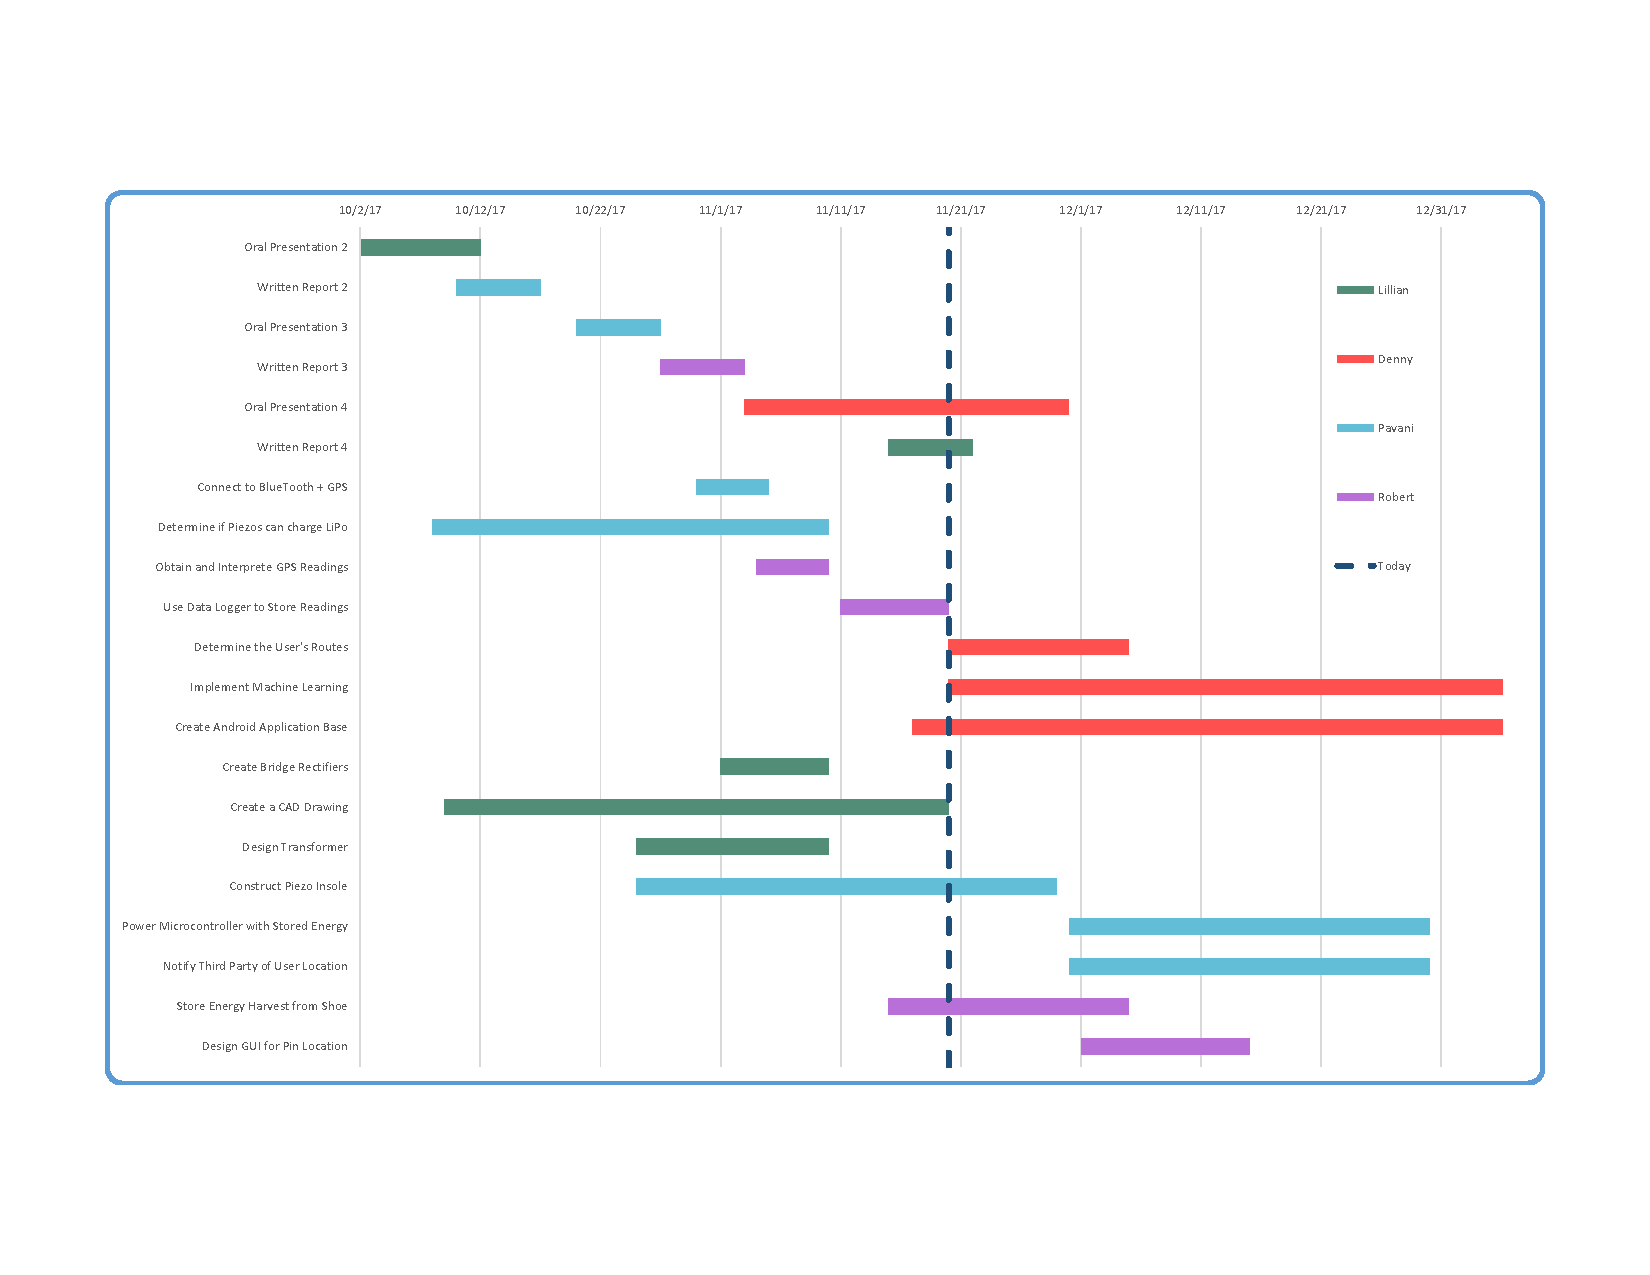
\includegraphics[trim=55 100 75 95, clip, width=\columnwidth]{GanttChart.pdf}
	\end{center}
	\vspace{-1em}
	\caption{\label{fig:Gantt}Gantt Chart for the rest of Fall Semester}
\end{figure}

\subsection{Objectives Accomplished}\label{sec:Accomplished}
In the previous months of work, the team has been able to complete all tasks on time as scheduled in previous Gantt charts. These were mainly research based tasks including researching kinetic energy harvesters, determining low power thresholds, and purchasing relevant parts. 

However there have been many design based tasks that have been accomplished including generating CAD models for sole specifications, creating possible circuit configurations for transformers, and making sensor placement mark-ups for their in-shoe placement. For these, actual shoes were studied and a CAD model was created based on the measurements of a size 12 shoe. This CAD model was then used toe create mark-ups of where piezoceramic disks would be placed based on Dr. Scholl's foot pressure point map.

\subsection{Objectives in Progress}\label{sec:inProgress}
From these research and design based tasks, we have moved to the testing stage for each of the components and circuit designs to test the efficiency and of each. In Figs. \ref{fig:Current} \& \ref{fig:Voltage} the measured values of voltage and current generate from the piezoceramic disks can seen plotted on the same axis with different configurations to compare their raw values. For all of these tests, 4 piezoceramic disks were sandwiched between insulating foam and hit twenty times to see the raw values they produced. These disks were tested in 3 different combinations, series, parallel, or a combination of the two. For both current and voltage, the values for the combination of series and parallel elements created the largest value. 

\begin{figure}[h]
	\begin{center}
		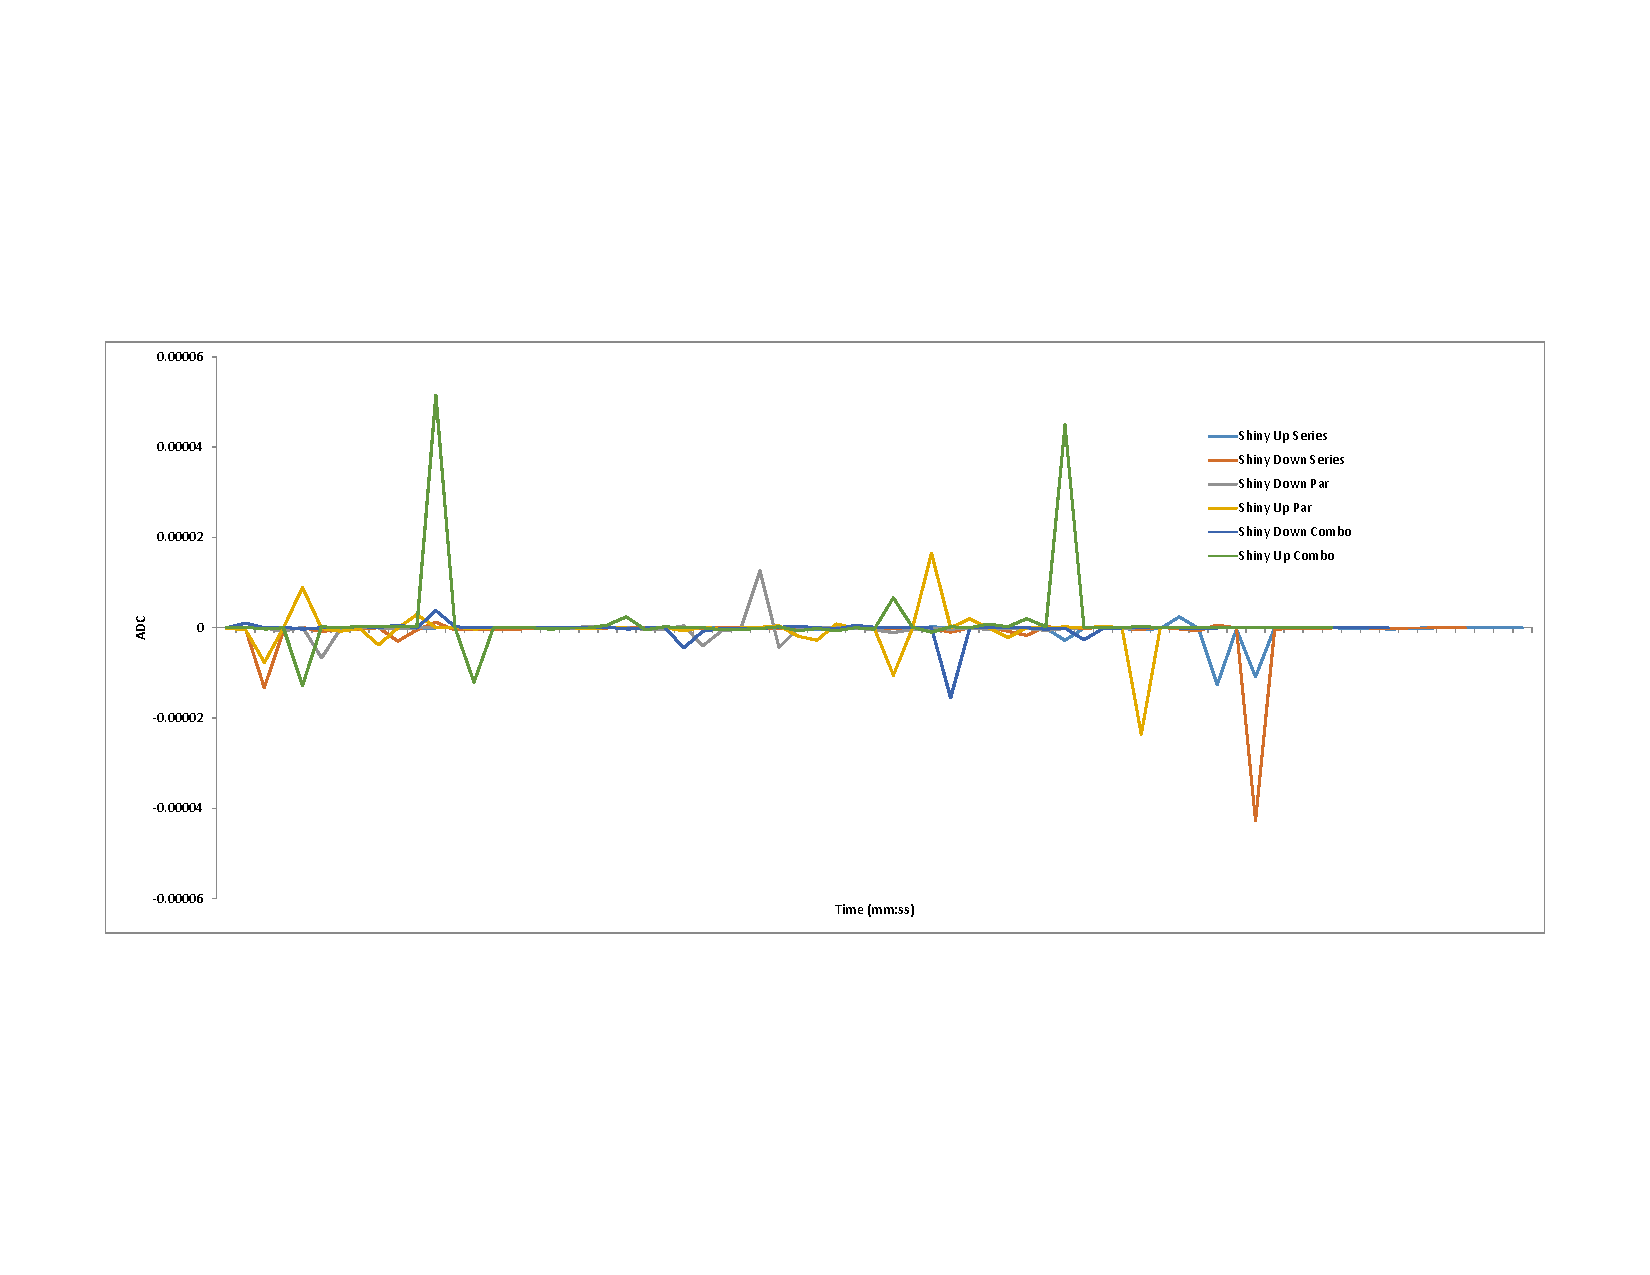
\includegraphics[trim=55 200 75 165, clip, width=\columnwidth]{Current.pdf}
	\end{center}
	\vspace{-1em}
	\caption{\label{fig:Current}Current readings from 4 piezoceramic sensors in 6 different combinations}
\end{figure}

\begin{figure}[h]
	\begin{center}
		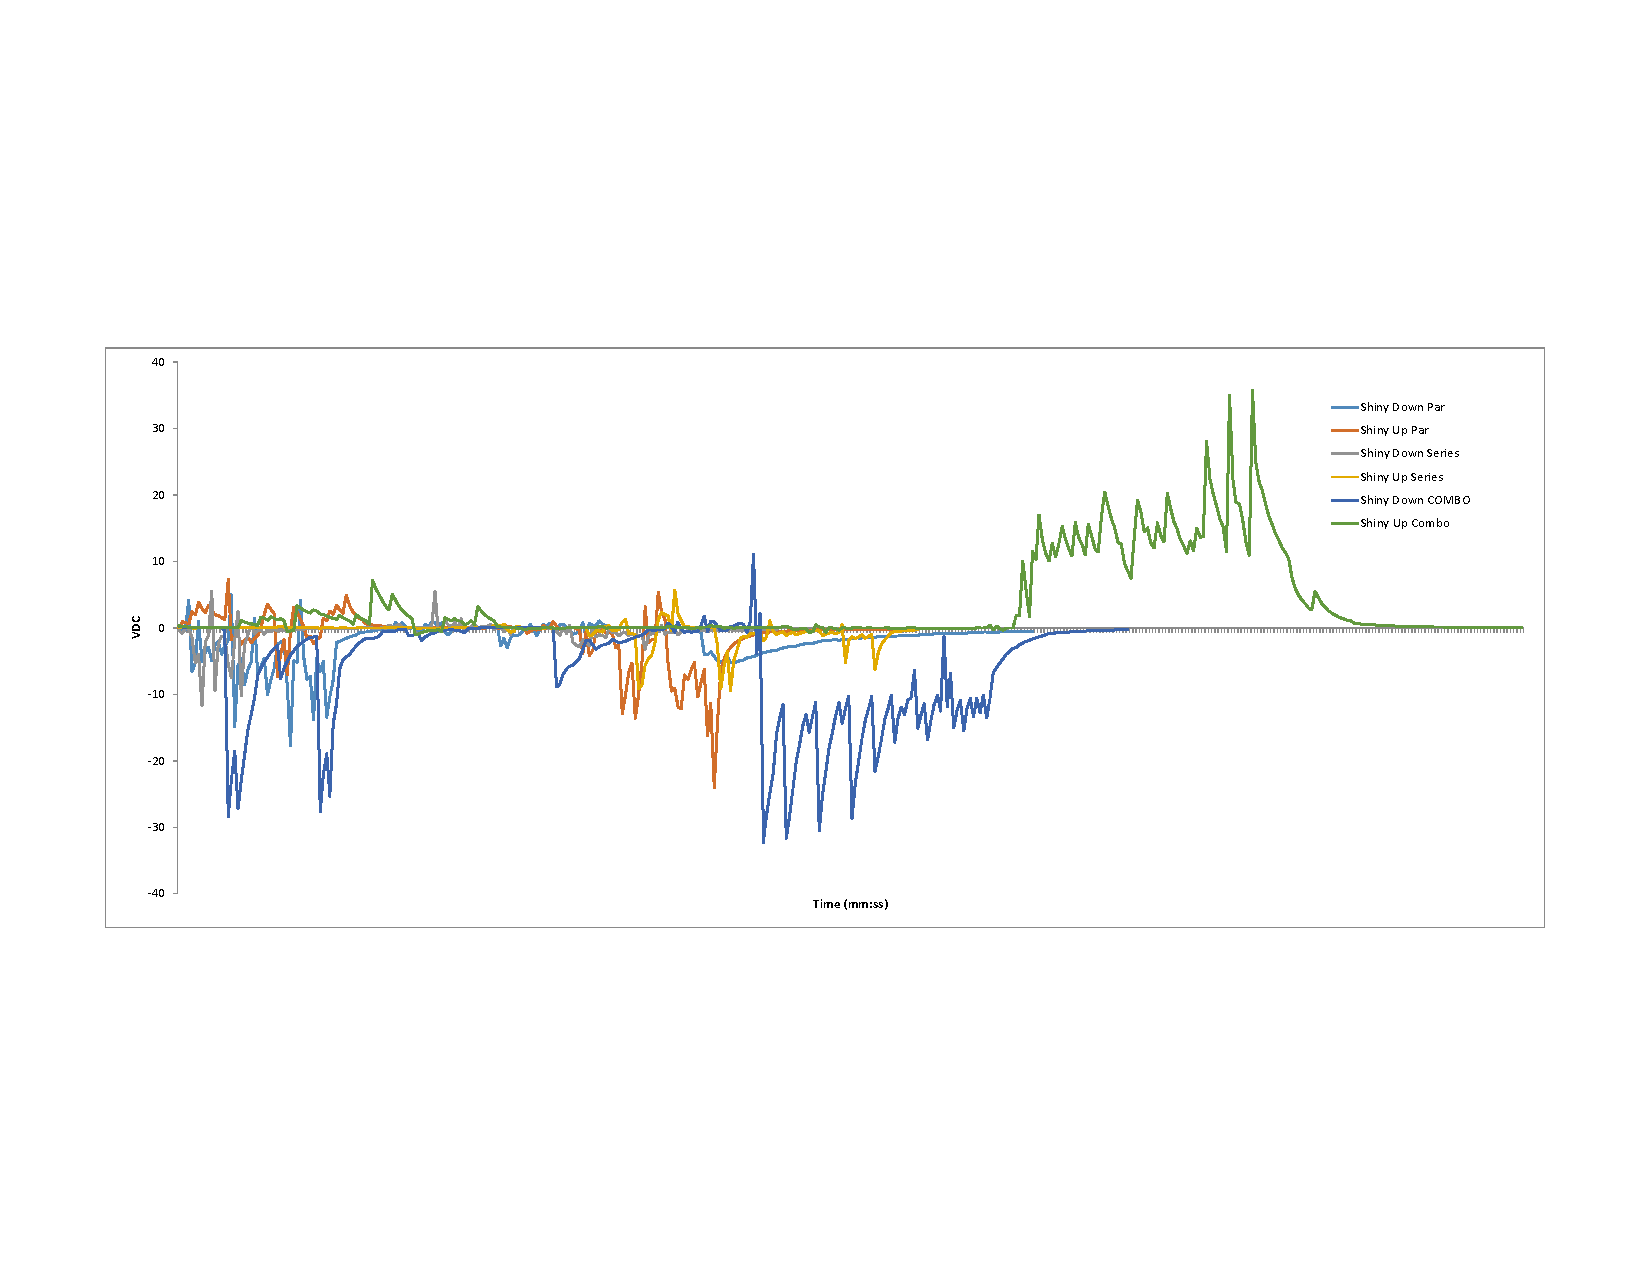
\includegraphics[trim=55 200 75 170, clip, width=\columnwidth]{Voltage.pdf}
	\end{center}
	\vspace{-1em}
	\caption{\label{fig:Voltage}Voltage readings from 4 piezoceramic sensors in 6 different combinations}
\end{figure}

Using the ideal combination of piezoceramic disks as seen in these two graphs, we will be testing transformer circuit configurations to determine which circuit is the most efficient at transferring the energy being generated into the energy bank, which for our testing purposes will be a capacitor. While preliminary tests have been run, the amount of noise being found in the tests have made the current data uncertain. From these tests, we will determine the proper placement for the piezoceramic disks inside the shoe for the maximum energy generation.

We have also began to test the ability to connect our sensors to our microprocessor and how much energy the total circuit will be drawing. While we have an approximate energy draw of 75 milliwatts, we have been considering even more low powered devices to decrease this draw further as Figs. \ref{fig:Current} \& \ref{fig:Voltage} do not approximate a large enough average wattage to power these electronics consistently enough.

\subsection{Objectives Remaining}\label{sec:Remaining}
The rest of this semester efforts will mainly focus on continuing tests for the circuit design with the main goal for the fall semester culminating into the ability to transfer the energy currently being stored in the energy bank into the microprocessor. We would also like a basic phone application that can read the sensor values from a microprocessor in ideal settings set up prior to connecting the processor and sensors to our unideal energy source.

\section{Budget}\label{sec:Budget}
In Table \ref{table:Labor}, the approximate cost in labor and consulting for the project can be seen. Although no one is currently being paid for the project we assume that each team member would earn a rate of \$50/hour and each team member would spend approximately 25 hours a week for the 16 weeks the project will cover.

\begin{table}[h!]
	\caption{\label{table:Labor}Labor and Consulting Budget}
	\begin{center}
		\begin{tabular}{ c|r c c r } 
			Item & Projected Cost & Cost/rate & Amount & Actual Cost \\
			\hline
			Workers & \$64,000.00 & \$50/hr & 380 & \$19,000.00 \\ 
			Consulting & \$2,500.00 & \$100/hr & 3.5 & \$350.00 \\ 
			\hline
			Total & \$66,500.00 &  &  & \$19,350.00 \\
		\end{tabular}
	\end{center}
\end{table}

The total cost of the shoe, seen in Table \ref{table:Components}, is projected to be around \$250. While this is considered to be a more expensive price for a pair of shoes, this is not an unreasonable price for a pair of shoes. As these shoes will also have advance technology inside of them and the possible mass production of the shoes when put on the market creates a lower price, the estimated cost of the shoes remains within a reasonable range.

\begin{table}[h!]
	\caption{\label{table:Components}Components Budget}
	\begin{center}
		\begin{tabular}{ c|r c c r } 
			Item & Projected Cost & Cost/rate & Amount & Actual Cost \\
			\hline
			Microprocessor & \$30.00 & \$19.80/unit & 2 & \$39.00 \\ 
			Piezoceramics & \$50.00 & \$1.00/sensor & 48 & \$48.00 \\ 
			Bluetooth & \$30.00 & \$39.95/sensor & 1 & \$39.95 \\ 
			GPS & \$20.00 & \$17.50/sensor & 1 & \$17.50 \\ 
			Shoe & \$80.00 & 0/pair & 1 & 0.00 \\ 
			Battery & \$40.00 & \$15.00/hr & 1 & \$15.00 \\ 
			\hline
			Total & \$250.00 &  &  & \$160.05 \\
		\end{tabular}
	\end{center} 
\end{table}

\section{Risk Management}\label{sec:Risk}
I have not yet killed Denny so that's a risk we've very successfully minimized.

\section{Conclusion}\label{sec:Conclusion}
The first semester for project stride is intended to focus on hardware and design issues. While we have encountered minor setbacks in the power specifications of our microprocessor and sensor modules from the our expected power output to our actual, we have not encountered any major setbacks from this and should continue on schedule to reach our target objectives at the end of the academic year.
    
\section*{Acknowledgements}
Project Stride would like to thank Doug Verret for his valuable input an guidance as the project sponsor as well as the Dr Steven Pei for leading the class as section facilitator.

\end{document}